\documentclass[a4paper]{article}

\def\nbook {All of Statistics: A Concise Course in Statistical Inference}
\def\nbookshort {All of Statistics}

% Shared preamble. The fallback lets the document build whether the working
% directory is its own folder or the project root.
\IfFileExists{header.tex}{\input{header}}{%%%%%%%%%%%%%%%%%%%%
% AUTHOR AND HEADER
% define \nbook
%%%%%%%%%%%%%%%%%%%%

\makeatletter
\ifx \nauthor\undefined
  \def\nauthor{David A. Lee}
\else
\fi

\author{\nbook \\ \small Solutions by \nauthor}
\date{}

%%%%%%%%%%%%%%%%%%%%
% PACKAGES
%%%%%%%%%%%%%%%%%%%%

\usepackage{alltt} 
\usepackage{amsfonts}
\usepackage{amsmath}
\usepackage{amssymb}
\usepackage{amsthm}
\usepackage{bm}
\usepackage{booktabs}
\usepackage{caption}
\usepackage{centernot}
\usepackage{enumitem}
\usepackage{fancyhdr}
\usepackage[T1]{fontenc}
\usepackage{graphicx}
% Images live in chap1/ ... chap8/ at the project root, while the documents that
% use them sit one level down (allofstats/, allofstatschap1/, ...). Listing both
% "./" and "../" lets a document keep writing \includegraphics{chap1/foo.eps}
% and still resolve it whether it is compiled from its own folder or from the
% project root.
\graphicspath{{./}{../}}
\usepackage{mathdots}
\usepackage{mathtools}
\usepackage{microtype}
\usepackage{multirow}
\usepackage{pdflscape}
\usepackage{pgfplots}
\pgfplotsset{compat=1.18}
\usepackage{siunitx}
\usepackage{slashed}
\usepackage{tabularx}
\usepackage{tikz}
\usepackage{titletoc}
\usepackage{tkz-euclide}
\usepackage[normalem]{ulem}
\usepackage{url}
\usepackage[all]{xy}
\usepackage{imakeidx}

% fonts
% use \textsf to change to Computer Modern Bright
\renewcommand{\sfdefault}{cmbr} % keeps default font Computer Modern Roman

% makeindex for table of contents
\makeindex[intoc, title=Index]
\indexsetup{othercode={\lhead{ Index }}}

% table of contents remove numbering
\setcounter{secnumdepth}{0}

% pagestyle
\pagestyle{fancyplain}

% header
\lhead{	\nouppercase{\leftmark} }
\ifx \nextra \undefined
  \rhead{
    \ifnum\thepage=1
    \else
      \nbookshort \  | \nauthor
    \fi}
\else
  \rhead{
    \ifnum\thepage=1
    \else
      \nbookshort (\nextra)
    \fi}
\fi

% proof environment

\newcommand{\prooffont}{\scshape}
\usepackage{xpatch}
\tracingpatches
\xpatchcmd{\proof}{\itshape}{\prooffont}{}{}

% Python environment (for typesetting Python code)

% Default fixed font does not support bold face
\DeclareFixedFont{\ttb}{T1}{txtt}{bx}{n}{8} % for bold
\DeclareFixedFont{\ttm}{T1}{txtt}{m}{n}{8}  % for normal

% Custom colors
\usepackage{color}
\definecolor{deepblue}{rgb}{0,0,0.5}
\definecolor{deepred}{rgb}{0.6,0,0}
\definecolor{deepgreen}{rgb}{0,0.5,0}

\usepackage{listings}

% Python style for highlighting
\newcommand\pythonstyle{\lstset{
language=Python,
basicstyle=\ttm,
morekeywords={self},              % Add keywords here
keywordstyle=\ttb\color{deepblue},
emph={MyClass,__init__},          % Custom highlighting
emphstyle=\ttb\color{deepred},    % Custom highlighting style
stringstyle=\color{deepgreen},
frame=tb,                         % Any extra options here
showstringspaces=false
}}


% Python environment
\lstnewenvironment{python}[1][]
{
\pythonstyle
\lstset{#1}
}
{}

% Python for external files
\newcommand\pythonexternal[2][]{{
\pythonstyle
\lstinputlisting[#1]{#2}}}

% Python for inline
\newcommand\pythoninline[1]{{\pythonstyle\lstinline!#1!}}

%%%%%%%%%%%%%
% FUNCTIONS %
%%%%%%%%%%%%%

\DeclarePairedDelimiter\abs{\lvert}{\rvert}%
\DeclarePairedDelimiter\norm{\lVert}{\rVert}%

%%%%%%%%%%%%%%%%%%%%
% DOCUMENT GEOMETRY
%%%%%%%%%%%%%%%%%%%%

\ifx \ntrim \undefined
\else
  \usepackage{geometry}
  \geometry{
	  papersize={379pt, 699pt},
	  textwidth=345pt,
	  left=17pt,
	  top=54pt,
	  right=17pt,
  }
\fi

% maketitle statement
\title{}
\ifx \nisofficial \undefined
\let\@real@maketitle\maketitle
\renewcommand{\maketitle}{\@real@maketitle\begin{center}\begin{minipage}[c]{0.9\textwidth}\centering\footnotesize All errors, typographical and substantive, and other offenses, are entirely my own.\end{minipage}\end{center}}
\else
\fi

%%%%%%%%%%%%%%%%%%%%
% THEOREMS
%%%%%%%%%%%%%%%%%%%%

%\theoremstyle{definition}
\newtheorem*{axiom}{Axiom}
\newtheorem*{claim}{Claim}
\newtheorem*{conjecture}{Conjecture}
\newtheorem*{cor}{Corollary}
%\newtheorem*{dfn}{Definition}
\newtheorem*{eg}{Example}
\newtheorem*{ex}{Exercise}
%\newtheorem*{lemma}{Lemma}
\newtheorem*{prop}{Proposition}
%\newtheorem*{thm}{Theorem}
\newtheorem*{remark}{Remark}
\newtheorem*{warning}{Warning}

%%%%%%%%%%%%%%%%%%%%
% FORMATTING AESTHETICS
%%%%%%%%%%%%%%%%%%%%

% itemize bullets
\renewcommand{\labelitemi}{-}
\renewcommand{\labelitemii}{$\circ$}
\renewcommand{\labelenumi}{(\roman{*})}

% new page section
\let\stdsection\section
\renewcommand\section{\newpage\stdsection}

%%%%%%%%%%%%%%%%%%%%
% \mathbb commands
%%%%%%%%%%%%%%%%%%%%

\newcommand{\C}{\mathbb{C}}
\newcommand{\N}{\mathbb{N}}
\newcommand{\Q}{\mathbb{Q}}
\newcommand{\R}{\mathbb{R}}
\newcommand{\Z}{\mathbb{Z}}


%%%%%%%%%%%%%%%%%%%%
% Probability Operators
%%%%%%%%%%%%%%%%%%%%

\DeclareMathOperator{\Bernoulli}{Bernoulli}
\DeclareMathOperator{\betaD}{Beta}
\DeclareMathOperator{\bias}{\textsf{bias}}
\DeclareMathOperator{\binomial}{Binomial}
\DeclareMathOperator{\corr}{Corr}
\DeclareMathOperator{\cov}{\textsf{Cov}}
\DeclareMathOperator{\Exp}{Exp}
\DeclareMathOperator{\gammaD}{Gamma}
\DeclareMathOperator{\mse}{\textsf{MSE}}
\DeclareMathOperator{\multinomial}{Multinomial}
\DeclareMathOperator{\Poisson}{Poisson}
\DeclareMathOperator{\sd}{sd}
\DeclareMathOperator{\se}{\textsf{se}}
\DeclareMathOperator{\Uniform}{Uniform}
\newcommand{\Prob}{\mathbb{P}}
\newcommand{\var}{\mathbb{V}}
\newcommand{\E}{\mathbb{E}}

%%%%%%%%%%%%%%%%%%%%
% TCOLORBOX CODE FROM SeniorMars
%%%%%%%%%%%%%%%%%%%%

%\usepackage[varbb]{newpxmath} changes math font to newpxmath
\usepackage{xfrac}
\usepackage[makeroom]{cancel}
\usepackage{mathtools}
\usepackage{bookmark}
\usepackage{enumitem}
\usepackage{hyperref,theoremref}
\hypersetup{
	pdftitle={Assignment},
	colorlinks=true, linkcolor=doc!90,
	bookmarksnumbered=true,
	bookmarksopen=true
}
\usepackage[most,many,breakable]{tcolorbox}
\usepackage{xcolor}
\usepackage{varwidth}
\usepackage{varwidth}
\usepackage{etoolbox}
%\usepackage{authblk}
\usepackage{nameref}
\usepackage{multicol,array}
\usepackage{tikz-cd}
\usepackage[ruled,vlined,linesnumbered]{algorithm2e}
\usepackage{comment} % enables the use of multi-line comments (\ifx \fi)
\usepackage{import}
\usepackage{xifthen}
\usepackage{pdfpages}
\usepackage{transparent}

\newcommand\mycommfont[1]{\footnotesize\ttfamily\textcolor{blue}{#1}}
\SetCommentSty{mycommfont}
\newcommand{\incfig}[1]{%
    \def\svgwidth{\columnwidth}
    \import{./figures/}{#1.pdf_tex}
}

\usepackage{tikzsymbols}

% colors -- change them as you may!

\definecolor{myg}{RGB}{56, 140, 70}
\definecolor{myb}{RGB}{45, 111, 177}
\definecolor{myr}{RGB}{199, 68, 64}
\definecolor{mytheorembg}{HTML}{F2F2F9}
\definecolor{mytheoremfr}{HTML}{00007B}
\definecolor{mylenmabg}{HTML}{FFFAF8}
\definecolor{mylenmafr}{HTML}{983b0f}
\definecolor{mypropbg}{HTML}{f2fbfc}
\definecolor{mypropfr}{HTML}{191971}
\definecolor{myexamplebg}{HTML}{F2FBF8}
\definecolor{myexamplefr}{HTML}{88D6D1}
\definecolor{myexampleti}{HTML}{2A7F7F}
\definecolor{mydefinitbg}{HTML}{E5E5FF}
\definecolor{mydefinitfr}{HTML}{3F3FA3}
\definecolor{notesgreen}{RGB}{0,162,0}
\definecolor{myp}{RGB}{197, 92, 212}
\definecolor{mygr}{HTML}{880808}
\definecolor{myred}{RGB}{127,0,0}
\definecolor{myyellow}{RGB}{169,121,69}
\definecolor{myexercisebg}{HTML}{F2FBF8}
\definecolor{myexercisefg}{HTML}{88D6D1}
\definecolor{doc}{RGB}{0,60,110}

%================================
% THEOREM BOX
%================================

%\providecommand\theoremnumber{}
\tcbuselibrary{theorems,skins,hooks}
\newtcbtheorem{Theorem}{Theorem}
{%
	enhanced,
	breakable,
	colback = mytheorembg,
	frame hidden,
	boxrule = 0sp,
	borderline west = {2pt}{0pt}{mytheoremfr},
	sharp corners,
	detach title,
	before upper = \tcbtitle\par\smallskip,
	coltitle = mytheoremfr,
	fonttitle = \bfseries\sffamily,
	description font = \mdseries,
	separator sign none,
	segmentation style={solid, mytheoremfr},
}
{th}


%================================
% Question BOX
%================================

\makeatletter
\newtcbtheorem{question}{Question}{enhanced,
	breakable,
	colback=white,
	colframe=mygr,
	attach boxed title to top left={yshift*=-\tcboxedtitleheight},
	fonttitle=\bfseries\sffamily,
	title={#2},
	boxed title size=title,
	boxed title style={%
			sharp corners,
			rounded corners=northwest,
			colback=tcbcolframe,
			boxrule=0pt,
		},
	underlay boxed title={%
			\path[fill=tcbcolframe] (title.south west)--(title.south east)
			to[out=0, in=180] ([xshift=5mm]title.east)--
			(title.center-|frame.east)
			[rounded corners=\kvtcb@arc] |-
			(frame.north) -| cycle;
		},
	#1
}{def}
\makeatother

%================================
% PROPERTIES BOX
%================================

\tcbuselibrary{theorems,skins,hooks}
\newtcbtheorem{Property}{Property}
{%
	enhanced,
	breakable,
	colback = mytheorembg,
	frame hidden,
	boxrule = 0sp,
	borderline west = {2pt}{0pt}{mytheoremfr},
	sharp corners,
	detach title,
	before upper = \tcbtitle\par\smallskip,
	coltitle = mytheoremfr,
	fonttitle = \bfseries\sffamily,
	description font = \mdseries,
	separator sign none,
	segmentation style={solid, mytheoremfr},
}
{th}

%================================
% LEMMA
%================================

\tcbuselibrary{theorems,skins,hooks}
\newtcbtheorem[number within=section]{Lemma}{Lemma}
{%
	enhanced,
	breakable,
	colback = mylenmabg,
	frame hidden,
	boxrule = 0sp,
	borderline west = {2pt}{0pt}{mylenmafr},
	sharp corners,
	detach title,
	before upper = \tcbtitle\par\smallskip,
	coltitle = mylenmafr,
	fonttitle = \bfseries\sffamily,
	description font = \mdseries,
	separator sign none,
	segmentation style={solid, mylenmafr},
}
{th}


% Commands for special boxes
\newcommand{\thm}[2]{\begin{Theorem*}{#1}{}#2\end{Theorem*}}
\newcommand{\qs}[2]{\begin{question*}{#1}{}#2\end{question*}}
\newcommand{\prp}[2]{\begin{Property*}{#1}{}#2\end{Property*}}
\newcommand{\lemma}[2]{\begin{Lemma*}{#1}{}#2\end{Lemma*}}
}

\begin{document}
\maketitle

\section{Chapter 7: Estimating the \textsf{CDF} and Statistical Functionals}

\subsection*{Import Packages}

Please see the associated GitHub repo for all code and comments to simulations. [LINK HERE]

\begin{python}
import numpy as np
from numpy.random import choice
import random
import matplotlib.pyplot as plt
import scienceplots
\end{python}

% QUESTION 1
\qs{7.4.1}{Prove Theorem 7.3.}
\thm{(Wasserman 7.3)}{At any fixed value of \(x\),
\begin{align*}
	\E\left( \widehat{F}_{n} \left( x \right)  \right) \quad & = \quad F \left( x \right), \\
	\var\left( \widehat{F}_{n} \left( x \right)  \right) \quad & = \quad \frac{F\left( x \right) \left( 1 - F\left( x \right) \right) }{n}, \\
	\mse \quad & = \quad \frac{F\left( x \right) \left( 1 - F\left( x \right) \right) }{n} \rightarrow 0, \\
	\widehat{F}_{n} \left( x \right) \quad  &\xrightarrow{\text{ P }} F\left( x \right).
\end{align*}}
\begin{proof}[Proof] 
\underline{\(\E\left( \widehat{F}_{n} \left( x \right)  \right) = F \left( x \right) \):}

By the definition of \(\widehat{F}_{n} \left( x \right) \), we have
\begin{align*}
	\E\left( \widehat{F}_{n} \left( x \right)  \right) & = \E\left( \frac{\sum_{i=1}^{n} I \left( X_{i} \le x \right) }{n} \right) \\
	 & = \frac{1}{n} \sum_{i=1}^{n} \Prob\left( X_{i} \le x  \right) \\ 
	 & = \frac{1}{n} \left( n F \left( x \right)  \right) \\
	 & = F \left( x \right) 
\end{align*}

\underline{\(\var\left( \widehat{F}_{n} \left( x \right)  \right) = F \left( x \right) \left( 1 - F \left( x \right)  \right) / n\):}

\begin{align*}
	\var\left( \widehat{F}_{n}\left( x \right)  \right) & = \E\left( \widehat{F}^{2}_{n}\left( x \right)  \right) - \E\left( \widehat{F}_{n} \left( x \right)  \right)^{2} \\
	 & = \E\left( \frac{1}{n^{2}} \left( \sum_{i=1}^{n} I \left( X_{i} \le x \right)  \right)^{2} \right) - F \left( X \right)^{2} \\ 
	 & = \frac{1}{n^{2}} \E\left( \sum_{j=1}^{n} \sum_{i=1}^{n} I \left( X_{j} \le x \right) I \left( X_{i} \le x \right)  \right) - F \left( x \right)^{2} \\
	 & = \frac{1}{n^{2}} \left( \sum_{i=1}^{n} \Prob\left( X_{i} \le x \right) + \sum_{j=1}^{n} \sum_{\substack{i = 1 \\ i \neq j}}^{n} \Prob\left( X_{j} \le x \right) \Prob\left( X_{i} \le x \right) \right)  - F \left( x \right)^{2}\\
	 & = \frac{1}{n^{2}} \left( n F \left( x \right) + n \left( n - 1 \right) F \left( x \right)^{2} \right) - F \left( x \right)^{2} \\
	 & = \frac{F \left( x \right) + \left( n-1 \right) F \left( x \right)^{2} - n F \left( x \right)^{2}}{n} \\
	 & = \frac{F \left( x \right) \left( 1 - F \left( x \right)  \right) }{n}
\end{align*}

\underline{\(\mse = F \left( x \right) \left( 1 - F \left( x \right)  \right) / n \rightarrow 0\):}

\begin{align*}
	\mse  & = \bias^{2} \left( \widehat{F}_{n} \left( x \right)  \right) + \var\left( \widehat{F}_{n} \left( x \right)  \right) \\
	 & = \frac{F \left( x \right) \left( 1 - F \left( x \right)  \right) }{n} \rightarrow 0 \text{ as } n \rightarrow \infty \\ 
\end{align*}

\underline{\(\widehat{F}_{n} \left( x \right) \xrightarrow{\text{ P }} F \left( x \right) \) :}

Since
\[
	\E\left( \widehat{F}_{n} \left( x \right) - F \left( x \right)  \right)^{2} = \var\left( \widehat{F}_{n} \left( x \right)  \right) \rightarrow 0 \text{ as } n \rightarrow \infty
\]
It follows that \(\widehat{F}_{n} \left( x \right) \xrightarrow{\text{qm}} F \left( x \right) \), implying \(\widehat{F}_{n} \left( x \right)  \xrightarrow{\text{ P }} F \left( x \right) \).
\end{proof}

% QUESTION 2
\qs{7.4.2}{Let \(X_{1}, \dots, X_{n} \sim \Bernoulli\left( p \right)\) and let \(Y_{1}, \dots, Y_{m} \sim \Bernoulli\left( q \right)\). Find the plug-in estimator and estimated standard error for \(p\). Find an approximate 90 percent confidence interval for \(p\). Find the plug-in estimator and estimated standard error for \(p-q\). Find an approximate 90 percent confidence interval for \(p-q\).}

By Theorem 7.9,
\begin{align*}
	\widehat{p} & = \int x d \widehat{F}_{n} \left( x \right) = \boxed{\overline{X}_{n}} \\
	\widehat{\se } &  = \widehat{\sigma } / \sqrt{n} = \boxed{\sqrt{\frac{\widehat{p} \left( 1 - \widehat{p} \right) }{n}}} 
\end{align*}
The 90 percent confidence interval for \(p\) has \(z_{\alpha / 2} = z_{.1/2} = 1.65\), so we have
\[
	\boxed{ \overline{X}_{n} \pm 1.65 \sqrt{\frac{\widehat{p} \left( 1 - \widehat{p} \right) }{n}} }
\]
For \(p-q\), we have
\begin{align*}
	\widehat{p-q} & = \int x d \widehat{F}_{n} \left( x \right) - \int y d \widehat{F}_{n} \left( y \right) = \boxed{\overline{X}_{n} - \overline{Y}_{n}} \\
	\widehat{\se } & = \sqrt{\frac{\widehat{\sigma^{2}_{p}}}{n} + \frac{\widehat{\sigma^{2}_{q}}}{m}} = \boxed{\sqrt{\frac{\widehat{p} \left( 1 - \widehat{p} \right) }{n} + \frac{\widehat{q} \left( 1 - \widehat{q} \right) }{m}}} \\
	\text{90 percent CI:} & = \boxed{\overline{X}_{n} - \overline{Y}_{n} \pm 1.65 \widehat{\se}}
\end{align*}

% QUESTION 3
\qs{7.4.3}{\textsf{(Computer Experiment.)} Generate 100 observations from a \(N \left( 0,1 \right) \) distribution. Compute a 95 percent confidence band for the \textsf{CDF} \(F\). Repeat this 1000 times and see how often the confidence band contains the true distribution function. Repeat using data from a Cauchy distribution.}

Using the DKW inequality, we can construct the confidence band from a standard normal distribution in the following manner:

\begin{python}
n = 100
alpha = 0.05
eps = np.sqrt((1/(2*n))*np.log(2/alpha))

def ecdfhat(sample):
    cdfhat = [ i/len(sample) for i in range(1, len(sample)+1)]
    return cdfhat;

def dkwintnormal():
    dkwtest, lowerbound, upperbound = 
    	np.empty(n), np.empty(n), np.empty(n)
    sample = np.sort(np.random.normal(0,1,n))
    ecdf = ecdfhat(sample)
    for i,j in zip(range(0, len(sample)), sample):
        lowerbound[i] = max(ecdf[i] - eps, 0)
        upperbound[i] = min(ecdf[i] + eps, 1)
        dkwtest[i] = 
		(norm.cdf(j) >= lowerbound[i]) 
		& (norm.cdf(j) <= upperbound[i])
    return dkwtest, lowerbound, upperbound, ecdf, sample;
\end{python}

\begin{center}
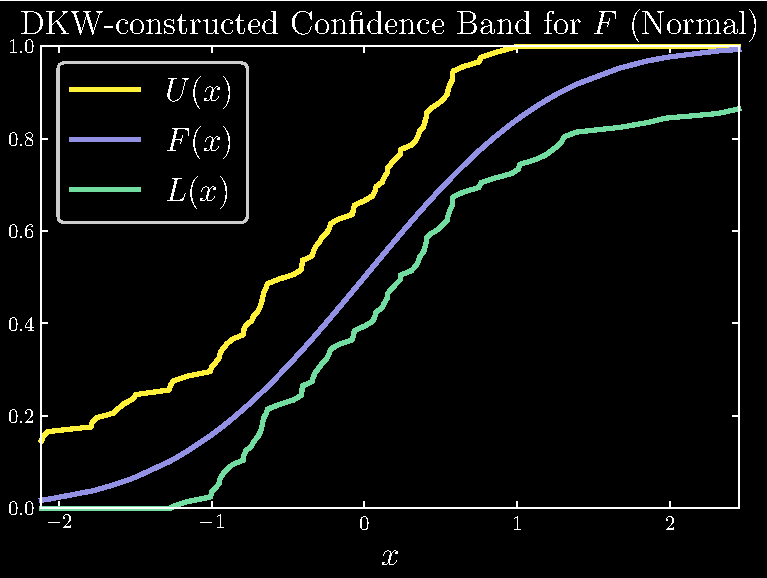
\includegraphics[width=1.0\textwidth]{chap7/chap7ex3i.eps}
\end{center}

The probability that the \textsf{CDF} \(F\) is contained in the confidence band approaches \(0.95\) for large number of iterations:

\begin{center}
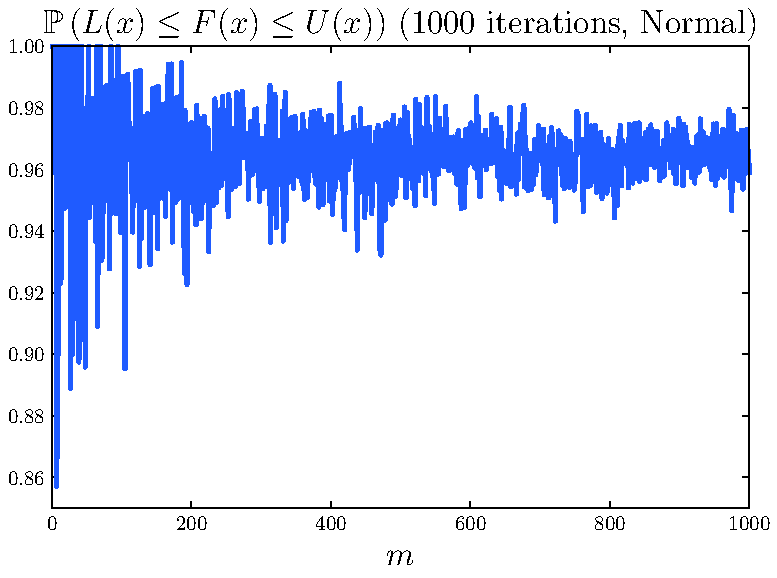
\includegraphics[width=1.0\textwidth]{chap7/chap7ex3ii.eps}
\end{center}

Repeating the same for data from a standard Cauchy distribution, we get:

\begin{python}
n = 100
alpha = 0.05
eps = np.sqrt((1/(2*n))*np.log(2/alpha))

def ecdfhat(sample):
    cdfhat = [ i/len(sample) for i in range(1, len(sample)+1)]
    return cdfhat;

def dkwintcauchy():
    dkwtest, lowerbound, upperbound = 
    	np.empty(n), np.empty(n), np.empty(n)
    sample = np.sort(np.random.standard_cauchy(n))
    ecdf = ecdfhat(sample)
    for i,j in zip(range(0, len(sample)), sample):
        lowerbound[i] = max(ecdf[i] - eps, 0)
        upperbound[i] = min(ecdf[i] + eps, 1)
        dkwtest[i] = 
		(norm.cdf(j) >= lowerbound[i]) 
		& (norm.cdf(j) <= upperbound[i])
    return dkwtest, lowerbound, upperbound, ecdf, sample;
\end{python}

\begin{center}
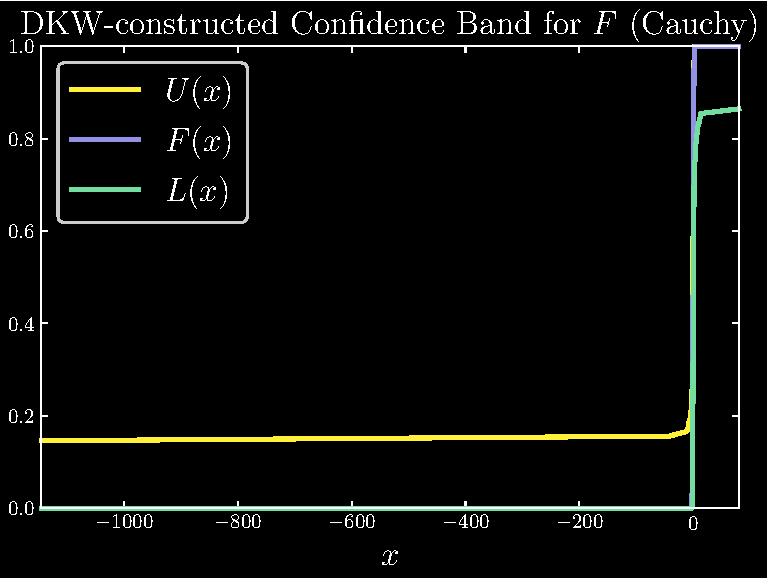
\includegraphics[width=1.0\textwidth]{chap7/chap7ex3iii.eps}
\end{center}

\begin{center}
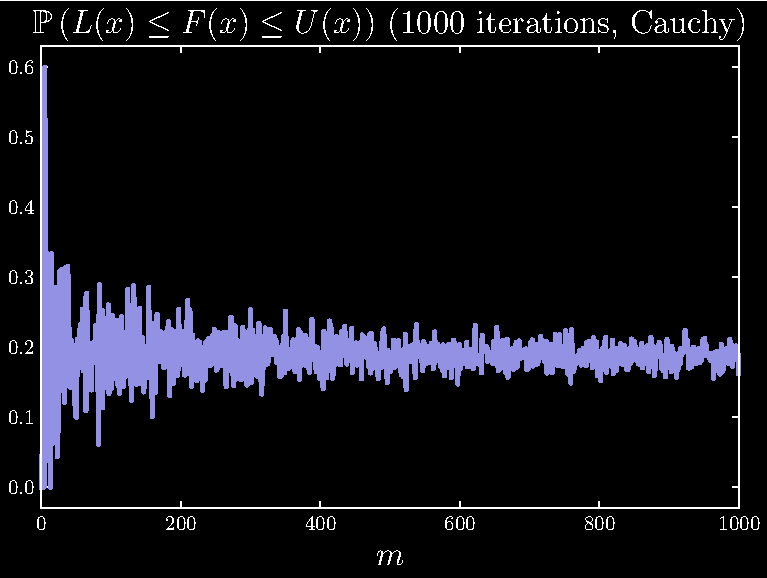
\includegraphics[width=1.0\textwidth]{chap7/chap7ex3iv.eps}
\end{center}

% QUESTION 4
\qs{7.4.4}{Let \(X_{1}, \dots, X_{n} \sim F\) and let \(\widehat{F}_{n} \left( x \right) \) be the empirical distribution function. For a fixed \(x\), use the central limit theorem to find the limiting distribution of \(\widehat{F}_{n} \left( x \right) \).}

Using Theorem 7.3 and the proof from exercise 7.4.1, by the Central Limit Theorem, we have
\[
	\widehat{F}_{n} \left( x \right) \approx N \left( F \left( x \right) , \frac{F \left( x \right) \left( 1 - F \left( x \right)  \right) }{n} \right) 
\]

\newpage
% QUESTION 5
\qs{7.4.5}{Let \(x\) and \(y\) be two distinct points. Find \( \cov\left( \widehat{F}_{n}\left( x \right) , \widehat{F}_{n} \left( y \right)  \right)\).}

By definition of covariance, we have \(\cov\left( \widehat{F}_{n} \left( x \right) , \widehat{F}_{n} \left( y \right)  \right)\) equal to:
\begin{align*}
	 & = \E\left( \left( \widehat{F}_{n}\left( x \right) - \E\left( \widehat{F}_{n}\left( x \right)  \right) \right) \left( \widehat{F}_{n}\left( y \right) - \E\left( \widehat{F}_{n}\left( y \right)  \right) \right)  \right) \\
	 & = \E\left( \left( \widehat{F}_{n}\left( x \right) - F \left( x \right)  \right) \left( \widehat{F}_{n}\left( y \right) - F \left( y \right)  \right)  \right)  \\ 
	 & = \E\left( \widehat{F}_{n}\left( x \right) \widehat{F}_{n}\left( y \right)  \right) - F \left( x \right) F \left( y \right) \\
	 & = \E\left( \frac{1}{n^{2}} \left( \sum_{i=1}^{n} I \left( X_{i} \le x \right)  \right) \left( \sum_{j=1}^{n} I \left( X_{j} \le y \right)  \right)  \right) - F \left( x \right) F \left( y \right) \\
	 & = \frac{1}{n^{2}} \E\left( \sum_{i=1}^{n} I \left( X_{i} \le x \right) I \left( X_{i} \le y \right) + \sum_{i=1}^{n} \sum_{\substack{j = 1 \\ j \neq i}}^{n} I \left( X_{i} \le x \right) I \left( X_{j} \le y \right)  \right) \\
	 & \quad - F \left( x \right) F \left( y \right) 
\end{align*}

Now, for the first term to have non-zero terms in the sum, we must have \(X_{i} \le x,y\). Since \(x,y\) are distinct, either \(x < y\) or \(y < x\). Suppose without loss of generality that \(x < y\). Then the first term resolves to
\[
	\E\left( \sum_{i=1}^{n} I \left( X_{i} \le x \right) I \left( X_{i} \le y \right)  \right) = n \Prob\left( X_{i} \le y \right) = n F \left( y \right) 
\]

For the second term, assuming independence, we have
\begin{align*}
	\E\left( \sum_{i=1}^{n} \sum_{\substack{j = 1 \\ j \neq i}}^{n} I \left( X_{i} \le x \right) I \left( X_{j} \le y \right)  \right) & = n \left( n-1 \right) \Prob\left( X_{i} \le x \right) \Prob\left( X_{j}<= y \right) \\
	 & = n \left( n-1 \right) F \left( x \right) F \left( y \right)  \\ 
\end{align*}

Combining the terms, we can conclude that the covariance is equal to
\begin{align*}
	 & = \frac{1}{n^{2}} \left( n F \left( y \right) + n \left( n - 1 \right) F \left( x \right) F \left( y \right)  \right) - F \left( x \right) F \left( y \right)  \\
	 & = \frac{F \left( y \right) + \left( n - 1 \right) F \left( x \right) F \left( y \right) - n F \left( x \right) F \left( y \right) }{n} \\ 
	 & = \boxed{\frac{F \left( y \right) \left( 1 - F \left( x \right)  \right) }{n}}
\end{align*}

% QUESTION 6
\qs{7.4.6}{Let \(X_{1}, \dots, X_{n} \sim F\) and let \(\widehat{F}\) be the empirical distribution function. Let \(a < b\) be fixed numbers and define \(\theta = T \left( F \right) = F \left( b \right) - F \left( a \right) \). Let \(\widehat{\theta} = T \left( \widehat{F}_{n} \right) = \widehat{F}_{n} \left( b \right) - \widehat{F}_{n} \left( a \right) \). Find the estimated standard error of \(\widehat{\theta}\). Find an expression for an approximate \(1 - \alpha \) confidence interval for \(\theta\).}

Using exercise 7.4.5, we can derive
\begin{align*}
	\var\left( \widehat{\theta} \right) & = \var\left( \widehat{F}_{n} \left( b \right) - \widehat{F}_{n} \left( a \right)  \right) \\
	 & = \var\left( \widehat{F}_{n} \left( b \right)  \right) + \var\left( \widehat{F}_{n} \left( a \right)  \right) + 2 \cov\left( \widehat{F}_{n} \left( b \right), \widehat{F}_{n}\left( a \right)  \right) \\
	 & = \frac{1}{n} \left( F \left( b \right) \left( 1 - F \left( b \right)  \right) + F \left( a \right) \left( 1 - F \left( a \right)  \right) + 2 F \left( b \right) \left( 1 - F \left( a \right)  \right)  \right) \\
	 & = \frac{1}{n} \left( F \left( b \right) - F \left( a \right)  \right) \left( 1 - \left( F \left( b \right) - F \left( a \right)  \right)  \right) \\
	\se \left( \widehat{\theta} \right) & = \sqrt{\var\left( \widehat{\theta} \right)} \\
	\widehat{\se } \left( \widehat{\theta} \right) & = \sqrt{\frac{1}{n} \left( \widehat{F}  \left( b \right) - \widehat{F} \left( a \right)  \right) \left( 1 - \left( \widehat{F} \left( b \right) - \widehat{F} \left( a \right)  \right)  \right)} \\
\end{align*}
The \(1 - \alpha \) confidence interval is given by
\[
	\widehat{\theta} \pm z_{\alpha /2} \widehat{\se} \left( \widehat{\theta} \right) 
\]

% QUESTION 7
\qs{7.4.7}{Data on the magnitudes of earthquakes near Fiji are available on the website for this book. Estimate the \textsf{CDF} \(F \left( x \right) \). Compute and plot a 95 percent confidence envelope for \(F\). Find an approximate 95 percent confidence interval for \(F \left( 4.9 \right) - F \left( 4.3 \right) \).}

The 95 percent confidence interval for \(F(4.9) - F(4.3)\) is \((0.495, 0.557)\).
The DKW-constructed confidence band for \(F\) is as follows:

\begin{python}
fijidata = pd.read_csv('fijiquakes.dat', delim_whitespace=True)

magdata = np.sort(fijidata['mag'])

n = len(magdata)
alpha = 0.05
eps = np.sqrt((1/(2*n))*np.log(2/alpha))

def ecdfhat(sample):
    cdfhat = [ i/len(sample) for i in range(1, len(sample)+1)]
    return cdfhat;

def dkwbounds():
    lowerbound, upperbound = 
    	np.empty(len(magdata)), 
	np.empty(len(magdata))
    ecdf = ecdfhat(magdata)
    for i in range(0, len(magdata)):
        lowerbound[i] = max(ecdf[i] - eps, 0)
        upperbound[i] = min(ecdf[i] + eps, 1)
    return lowerbound, upperbound;

# Use results of exercise 7.4.6 for confidence interval

theta = ecdf(4.9) - ecdf(4.3)
sehat = np.sqrt((1/len(magdata))*theta*(1-theta))
\end{python}

\begin{center}
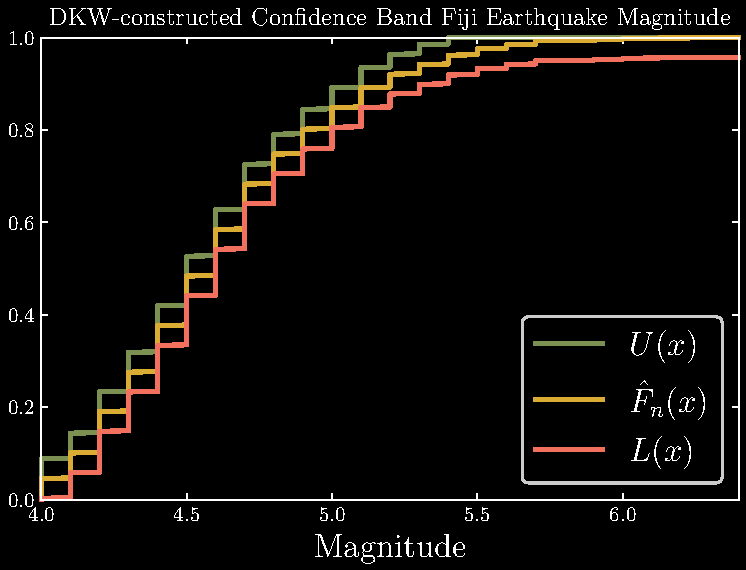
\includegraphics[width=1.0\textwidth]{chap7/chap7ex7.eps}
\end{center}

\newpage
% QUESTION 8
\qs{7.4.8}{Get the data on eruption times and waiting times between eruptions of the Old Faithful geyser from the website. Estimate the mean waiting time and give a standard error for the estimate. Also, give a 90 percent confidence interval for the mean waiting time. Now estimate the median waiting time. In the next chapter we will see how to get the standard error for the median.}

The estimated mean, standard error, 90 percent confidence interval, and median are \(70.897\), \(0.824\), \((69.537, 72.257)\), and \(76.0\), respectively.

\begin{python}
faithful = pd.read_csv('faithful.dat', delim_whitespace=True)
    
waitingdata = faithful['waiting']

waitingmean = np.mean(waitingdata)
waitingse = np.std(waitingdata, ddof=1) / np.sqrt(np.size(waitingdata))

waitingci = (round(waitingmean - 1.65*waitingse, 3), 
	     round(waitingmean + 1.65*waitingse, 3))

waitingmedian = np.median(waitingdata)
\end{python}


% QUESTION 9
\qs{7.4.9}{100 people are given a standard antibiotic to treat an infection and another 100 are given a new antibiotic. In the first group, 90 people recover; in the second group, 85 people recover. Let \(p_{1}\) be the probability of recovery under the standard treatment and let \(p_{2}\) be the probability of recovery under the new treatment. We are interested in estimating \(\theta = p_{1} - p_{2}\). Provide an estimate, standard error, an 80 percent confidence interval, and a 95 percent confidence interval for \(\theta\).}

We can model the odds of recovering as a Bernoulli variable. We estimate \(\widehat{\theta}\) as
\[
	\widehat{\theta} = \widehat{p_{1} - p_{2}} = \frac{90}{100} - \frac{85}{100} = \boxed{0.05}
\]
The estimate of the standard error is
\begin{align*}
	\widehat{\se }\left( \widehat{\theta} \right)  & = \sqrt{\frac{\widehat{p}_{1} \left( 1 - \widehat{p}_{1} \right) }{n} + \frac{\widehat{p}_{2} \left( 1 - \widehat{p}_{2} \right) }{n}} \\
	 & = \sqrt{\frac{90 / 100 \left( 1 - 90 / 100 \right) }{100} + \frac{85 / 100 \left( 1 - 85/100 \right) }{100}} \\ 
	 & \approx \boxed{0.0466}
\end{align*}

\underline{80 percent CI:} \(z_{\alpha /2} = z_{.2 / 2} = z_{0.1} \approx 1.28\)
\[
	0.05 \pm 0.0597
\]

\underline{95 percent CI:} \(z_{\alpha /2} = z_{0.05/2} = z_{0.025} \approx 1.96\)
\[
	0.05 \pm 0.0914
\]

% QUESTION 10
\qs{7.4.10}{In 1975, an experiment was conducted to see if cloud seeding produced rainfall. 26 clouds were seeded with silver nitrate and 26 were not. The decision to seed or not was made at random.

Let \(\theta\) be the difference in the mean precipitation from the two groups. Estimate \(\theta\). Estimate the standard error of the estimate and produce a 95 percent confidence interval.}

The estimates for \(\theta\), standard error, and the 95 percent confidence interval are \(277.396\), \(136.124\), and \((10.593, 544.199)\), respectively.

\begin{python}
clouds = pd.read_csv('clouds.dat', delim_whitespace=True)

unseeded = clouds['Unseeded_Clouds']
seeded = clouds['Seeded_Clouds']

diffmean = np.abs(np.mean(unseeded) - np.mean(seeded))
unseeded_se = np.std(unseeded) / np.sqrt(np.size(unseeded))
seeded_se = np.std(seeded) / np.sqrt(np.size(seeded))
diffse = np.sqrt(np.square(unseeded_se) + np.square(seeded_se))

diffci = (round(diffmean - 1.96*diffse, 3), 
	 round(diffmean + 1.96*diffse, 3))
\end{python}

\end{document}
